\documentclass[11pt,fleqn]{article}

\usepackage[T1]{fontenc}
\usepackage[utf8]{inputenc}
\usepackage[italian]{babel}

\usepackage{graphicx}
\usepackage{amsmath}
\usepackage{amssymb}
\usepackage{bm}
\usepackage[colorlinks]{hyperref}

\newcommand{\ul}[1]{\underline{#1}}
\newcommand{\uul}[1]{\ul{\ul{#1}}}
\newcommand{\p}[2]{\dfrac{\partial{#1}}{\partial{#2}}}
\newcommand{\f}[2]{\frac{#1}{#2}}
\newcommand{\bh}[1]{\bm{\hat{#1}}}
\newcommand{\remark}{}  % Dummy definition

\title{Alcuni chiarimenti su argomenti vari ed eventuali}

\begin{document}

\maketitle

\tableofcontents


\section{Traslazione, rotazione e deformazione e deformazione di un elemento di fluido}

Il moto di un elemento infinitesimo di fluido può essere descritto come composizione di una traslazione, di una rotazione rigida e una deformazione.
Siano $\bm{x}_1(t)$, $\bm{x}_2(t)$ le posizioni di due punti materiali e $\delta\bm{x}(t) = \bm{x}_2(t) - \bm{x}_1(t)$ il vettore che congiunge questi due punti.
La derivata temporale del vettore $\delta \bm{x}(t)$ può essere scritta come
\begin{equation}
 \frac{d \delta\bm{x}}{d t}(t) =
  \frac{d \bm{x}_2}{d t}(t) - \frac{d \bm{x}_1}{d t}(t) = 
  \bm{u}(\bm{x}_2(t),t) - \bm{u}(\bm{x}_1(t),t) \ , 
\end{equation}
avendo sfruttato la definizione di punto materiale per esprimere la sua velocità,
$d \bm{x}_i/dt$, come la velocità del continuo in quel punto, $\bm{u}(\bm{x}_i(t),t)$.
\newline \noindent
Utilizzando la definizione di $\delta \bm{x}(t)$, si può scrivere $\bm{x}_2(t) = \bm{x}_1(t) + \delta \bm{x}(t)$ ed esprimere la velocità calcolata in $\bm{x}_2(t)$ con un'espansione in serie centrata in $\bm{x}_1(t)$,
\begin{equation}
\begin{aligned}
    \bm{u}(\bm{x}_2(t),t) & = \bm{u}(\bm{x}_1(t)+\delta\bm{x}(t),t) = \\
    & = \bm{u}(\bm{x}_1(t),t) + \delta\bm{x}(t) \cdot \bm{\nabla} \bm{u}(\bm{x}_1(t),t) +
    o(|\delta\bm{x}(t)|) \ .
\end{aligned}
\end{equation}
Utilizzando la notazione tensoriale, si può quindi scrivere la derivata temporale di $\delta \bm{x}$ come
\begin{equation}\label{eqn:ddxdt:tens}
 \frac{d \delta \bm{x}}{d t}(t) = \delta \bm{x}(t) \cdot \bm{\nabla}\bm{u}(\bm{x}_1(t),t) + o(|\delta\bm{x}(t)|) \ .
\end{equation}
Utilizzando un sistema di coordinate cartesiane e la base naturale ortornormale $\{ \bm{\hat{x}}, \bm{\hat{y}}, \bm{\hat{z}} \}$, si può scrivere l'espressione (\ref{eqn:ddxdt:tens}) in componenti,
\begin{equation}
\begin{cases}
 \dfrac{d \delta x}{d t} =  x \p{u_x}{x} + y \p{u_x}{y} + z \p{u_x}{z} \\
 \dfrac{d \delta y}{d t} =  x \p{u_y}{x} + y \p{u_y}{y} + z \p{u_y}{z} \\
 \dfrac{d \delta z}{d t} =  x \p{u_z}{x} + y \p{u_z}{y} + z \p{u_z}{z} \\
\end{cases} \quad , \qquad 
 \dfrac{d \delta x_i}{d t} =  x_k \p{u_i}{x_k} 
\end{equation}


Il tensore del secondo ordine \textit{gradiente della velocità} $\bm{\nabla} \bm{u}$ può essere scritto come somma della sua parte simmetrica e della sua parte antisimmetrica, rispettivamente il \textit{tensore velocità di deformazione} $\mathbb{D}$ e \textit{tensore di spin} $\mathbb{R}$, $\bm{\nabla} \bm{u} = \mathbb{D} + \mathbb{W}$. Questi tensori possono essere scritti utilizzando la base prodotto costruita con i vettori della base cartesiana,
\begin{equation}\label{eqn:grad}
\begin{aligned}
 \bm{\nabla} \bm{u} = & \p{u_x}{x} \bm{\hat{x}}\otimes\bm{\hat{x}} + 
                        \p{u_x}{y} \bm{\hat{y}}\otimes\bm{\hat{x}} +
                        \p{u_x}{z} \bm{\hat{z}}\otimes\bm{\hat{x}} + \\
                    + & \p{u_y}{x} \bm{\hat{x}}\otimes\bm{\hat{y}} +
                        \p{u_y}{y} \bm{\hat{y}}\otimes\bm{\hat{y}} +
                        \p{u_y}{z} \bm{\hat{z}}\otimes\bm{\hat{y}} + \\
                    + & \p{u_z}{x} \bm{\hat{x}}\otimes\bm{\hat{z}} +
                        \p{u_z}{y} \bm{\hat{y}}\otimes\bm{\hat{z}} +
                        \p{u_z}{z} \bm{\hat{z}}\otimes\bm{\hat{z}}
\end{aligned} \hspace{1.0cm}
 \left\{ \bm{\nabla}\bm{u} \right\}_{ij} = \p{u_j}{x_i} \ ,
\end{equation}
\begin{equation}\label{eqn:d}
\begin{aligned}
 \mathbb{D} = & \frac{1}{2}\left[ \p{u_x}{x} +  \p{u_x}{x} \right] \bm{\hat{x}}\otimes\bm{\hat{x}} + 
                \frac{1}{2}\left[ \p{u_x}{y} +  \p{u_y}{x} \right] \bm{\hat{y}}\otimes\bm{\hat{x}} +
                \frac{1}{2}\left[ \p{u_x}{z} +  \p{u_z}{x} \right] \bm{\hat{z}}\otimes\bm{\hat{x}} + \\
            + & \frac{1}{2}\left[ \p{u_y}{x} +  \p{u_x}{y} \right] \bm{\hat{x}}\otimes\bm{\hat{y}} +
                \frac{1}{2}\left[ \p{u_y}{y} +  \p{u_y}{y} \right] \bm{\hat{y}}\otimes\bm{\hat{y}} +
                \frac{1}{2}\left[ \p{u_y}{z} +  \p{u_z}{y} \right] \bm{\hat{z}}\otimes\bm{\hat{y}} + \\
            + & \frac{1}{2}\left[ \p{u_z}{x} +  \p{u_x}{z} \right] \bm{\hat{x}}\otimes\bm{\hat{z}} +
                \frac{1}{2}\left[ \p{u_z}{y} +  \p{u_y}{z} \right] \bm{\hat{y}}\otimes\bm{\hat{z}} +
                \frac{1}{2}\left[ \p{u_z}{z} +  \p{u_z}{z} \right] \bm{\hat{z}}\otimes\bm{\hat{z}} \\
  D_{ij} & = \dfrac{1}{2}\left[ \p{u_j}{x_i} + \p{u_i}{x_j} \right] \ ,
\end{aligned}
\end{equation}
\begin{equation}\label{eqn:w}
\begin{aligned}
 \mathbb{W} = &  \hspace{2.0cm} 0 \hspace{0.5cm}                    \bm{\hat{x}}\otimes\bm{\hat{x}} + 
                \frac{1}{2}\left[ \p{u_x}{y} -  \p{u_y}{x} \right]  \bm{\hat{y}}\otimes\bm{\hat{x}} +
                \frac{1}{2}\left[ \p{u_x}{z} -  \p{u_z}{x} \right]  \bm{\hat{z}}\otimes\bm{\hat{x}} + \\
            + & \frac{1}{2}\left[ \p{u_y}{x} -  \p{u_x}{y} \right]  \bm{\hat{x}}\otimes\bm{\hat{y}} +
                 \hspace{2.0cm} 0 \hspace{0.5cm}                    \bm{\hat{y}}\otimes\bm{\hat{y}} +
                \frac{1}{2}\left[ \p{u_y}{z} -  \p{u_z}{y} \right]  \bm{\hat{z}}\otimes\bm{\hat{y}} + \\
            + & \frac{1}{2}\left[ \p{u_z}{x} -  \p{u_x}{z} \right]  \bm{\hat{x}}\otimes\bm{\hat{z}} +
                \frac{1}{2}\left[ \p{u_z}{y} -  \p{u_y}{z} \right]  \bm{\hat{y}}\otimes\bm{\hat{z}} +
                 \hspace{2.0cm} 0 \hspace{0.5cm}                    \bm{\hat{z}}\otimes\bm{\hat{z}} \\
  W_{ij} & = \dfrac{1}{2}\left[ \p{u_j}{x_i} - \p{u_i}{x_j} \right] \ .
\end{aligned}
\end{equation}
Osservando le componenti di $\mathbb{W}$, si possono riconoscere le componenti del campo \textit{vorticità} $\bm{\omega}$, definito come il rotore del campo di velocità, $\bm{\omega} = \bm{\nabla} \times \bm{u}$ e quindi scrivere,
\begin{equation}\label{eqn:w}
\begin{aligned}
 \mathbb{W} = & \ 0 \quad               \bm{\hat{x}}\otimes\bm{\hat{x}}   
              - \frac{1}{2} \omega_z \, \bm{\hat{y}}\otimes\bm{\hat{x}} +
                \frac{1}{2} \omega_y \, \bm{\hat{z}}\otimes\bm{\hat{x}} + \\
              & \frac{1}{2} \omega_z \, \bm{\hat{x}}\otimes\bm{\hat{y}} +
                \ 0 \quad               \bm{\hat{y}}\otimes\bm{\hat{y}}  
              - \frac{1}{2} \omega_x \, \bm{\hat{z}}\otimes\bm{\hat{y}} + \\
            - & \frac{1}{2} \omega_y \, \bm{\hat{x}}\otimes\bm{\hat{z}} +
                \frac{1}{2} \omega_x \, \bm{\hat{y}}\otimes\bm{\hat{z}} +
                \ 0 \quad               \bm{\hat{z}}\otimes\bm{\hat{z}} \\
\end{aligned}
\end{equation}

Ai tensori $\mathbb{D}$ e $\mathbb{W}$ si possono associare rispettivamente di deformazione e rotazione nell'evoluzione di $\delta \bm{x}(t)$,
\begin{equation}\label{eqn:evo:1}
    \frac{d \delta \bm{x}}{d t}(t) = \delta \bm{x}(t) \cdot \mathbb{D}(\bm{x}_1(t),t) +
                                     \delta \bm{x}(t) \cdot \mathbb{W}(\bm{x}_1(t),t) + o(|\delta\bm{x}(t)|) \ .
\end{equation}
Sfruttando la natura antisimmetrica del tensore di spin $\mathbb{W}$, si può riscrivere il contributo di rotazione al movimento in una forma che dovrebbe essere più familiare, corrispondente all'atto di moto rigido, visto in meccanica razionale. Aiutandosi con l'espressione del tensore $\mathbb{W}$ si può svolgere l'operazione $\delta\bm{x} \cdot \mathbb{W}$,
\begin{equation}
\begin{aligned}
 \delta\bm{x} \cdot \mathbb{W} & = \frac{1}{2}\left[ - \delta y \omega_z + \delta z \omega_y \right] \bm{\hat{x}} +
                                   \frac{1}{2}\left[ - \delta z \omega_x + \delta x \omega_z \right] \bm{\hat{y}} +
                                   \frac{1}{2}\left[ - \delta x \omega_y + \delta y \omega_x \right] \bm{\hat{z}} = \\
  & = \frac{1}{2} \bm{\omega} \times \delta \bm{x} \ ,
\end{aligned}
\end{equation}
avendo riconosciuto l'espressione del prodotto vettoriale tra $\bm{\omega}$ e $\delta \bm{x}$. L'equazione (\ref{eqn:evo:1}) può quindi essere riscritta,
\begin{equation}
    \frac{d \delta \bm{x}}{d t}(t) = \delta \bm{x}(t) \cdot \mathbb{D}(\bm{x}_1(t),t) + 
    \frac{1}{2} \bm{\omega}(\bm{x}_1(t),t) \times \delta \bm{x}(t) + o(|\delta\bm{x}(t)|) \ ,
\end{equation}
in modo tale da mettere in evidenza i due termini che determinano l'evoluzione del vettore elementare $\delta \bm{x}$:
\begin{itemize}
 \item il termine di rotazione ``media'', $\frac{1}{2} = \bm{\omega} \times \delta \bm{x}$; ricordando la legge dell'atto di moto rigido studiata in meccanica razionale,\footnote{
  Dati due punti $\bm{r}_1$, $\bm{r}_2$ appartenenti a un corpo rigido, vale la relazione
  % \begin{equation}
  %   \frac{d\bm{r}_2}{dt} - \frac{d\bm{r}_1}{dt} = \bm{\Omega} \times \left( \bm{r}_2 - \bm{r}_1 \right) \ ,
  % \end{equation}
  dove $\bm{\Omega}$ è il vettore velocità angolare del corpo rigido.
 }
 si può riconoscere il legame tra vorticità $\bm{\omega}$ e velocità angolare di una particella materiale: la vorticità $\bm{\omega}(\bm{x},t)$ risulta essere il doppio della velocità angolare della particella materiale che passa per il punto $\bm{x}$ all'istante temporale $t$.
 \item il termine di deformazione, $\mathbb{D} \cdot \delta \bm{x}$.\footnote{
 Poiché $\mathbb{D}$ è simmetrico, $\mathbb{D} \cdot \delta \bm{x} = \bm{x} \cdot \mathbb{D}$.}
\end{itemize}
%
 \noindent
L'evoluzione del punto materiale $\bm{x}_2(t)$ può quindi essere espressa in funzione del moto del punto $\bm{x}_1(t)$ e del vettore differenza $\delta\bm{x}_2(t)$,
\begin{equation}
\begin{aligned}
    \frac{d\bm{x}_2}{d t}(t) & = \ \frac{d\bm{x}_1}{d t}(t) + & \text{(traslazione)} \\
    & \ + \frac{1}{2} \bm{\omega}(\bm{x}_1(t),t) \times \delta \bm{x}(t) + & \text{(rotazione)} \\
    & \ + \delta \bm{x}(t) \cdot \mathbb{D}(\bm{x}_1(t),t) + & \text{(deformazione)} \\
    & \ + o(|\delta\bm{x}(t)|) & \text{(termini di ord.sup.)}
\end{aligned}
\end{equation}
riconoscendo i contributi di traslazione, rotazione, deformazione e contributi di ordine superiore che diventano trascurabili per $|\delta\bm{x}(t)| \rightarrow 0$.

\subsection{Esempio: corrente di Newton}
Si considera l'esempio della corrente di Newton in un canale piano infinito, descritta dal campo di velocità 
\begin{equation}
  \bm{u} = \frac{y}{H}U \bm{\hat{x}} \ .
\end{equation}
Si vuole determinare l'evoluzione in un istante di tempo $dt$ di due vettori materiali $\delta \bm{x}_a(t) = \bm{\hat{x}}$, $\delta \bm{x}_b(t) = \bm{\hat{y}}$, per valutare gli effetti di rotazione e deformazione di un volumetto elementare inizialmente quadrato, con i lati orientati come i due vettori considerati.
Si possono raccogliere le componenti cartesiane del gradiente di velocità $\bm{\nabla} \bm{u}$ nella matrice
\begin{equation}
 \left[
 \begin{array}{ccc} 
   u_x & u_y & u_z \\
   v_x & v_y & v_z \\
   w_x & w_y & w_z \\
 \end{array} \right] = 
 \left[
 \begin{array}{ccc} 
   0 & U/H & 0 \\
   0 &  0  & 0 \\
   0 &  0  & 0 \\
 \end{array} \right] \ ,
\end{equation}
e di conseguenza raccogliere le componenti dei tensori $\mathbb{D}$, $\mathbb{W}$ nelle matrici
\begin{equation}
 \uul{D} = 
 \left[
 \begin{array}{ccc} 
   0 & \frac{U}{2H} & 0 \\
   \frac{U}{2H} & 0 & 0 \\
   0 &  0  & 0 \\
 \end{array} \right] \quad , \quad
 \uul{W} = 
 \left[
 \begin{array}{ccc} 
   0 & \frac{U}{2H} & 0 \\
  -\frac{U}{2H} & 0 & 0 \\
   0 &  0  & 0 \\
 \end{array} \right] \ .
\end{equation}
All'istante $t+dt$, le componenti cartesiane $\ul{\delta x_i}(t+dt)$ vettore materiale $\delta \bm{x}_i(t+dt)$ possono essere ricavate come
\begin{equation}
 \begin{aligned}
     \ul{\delta x_i}(t+dt) & = \ul{\delta x_i}(t) + \frac{d \ul{\delta x_i}}{ dt}(t) = \\
     & = \ul{\delta x_i}(t) + \uul{D} \, \ul{\delta x_i} + 
                              \uul{W} \, \ul{\delta x_i} \ .
 \end{aligned}
\end{equation}
Svolgendo i conti per i vettori $\delta \bm{x}_a$, $\delta \bm{x}_b$, si ottiene,
\begin{equation}
 \begin{aligned}
     \ul{\delta x_a}(t+dt) & = \ul{\delta x_a}(t) +
     \left[ \begin{array}{c} 0 \\  \frac{U}{2H} \end{array}  \right] +
     \left[ \begin{array}{c} 0 \\ -\frac{U}{2H} \end{array}  \right] =
     \ul{\delta x_a}(t) =
     \left[ \begin{array}{c} 1 \\ 0 \end{array}  \right]
         \\
     \ul{\delta x_b}(t+dt) & = \ul{\delta x_b}(t) +
     \left[ \begin{array}{c} \frac{U}{2H} \\ 0 \end{array}  \right] +
     \left[ \begin{array}{c} \frac{U}{2H} \\ 0 \end{array}  \right] = 
     \ul{\delta x_a}(t) + 
     \left[ \begin{array}{c} \frac{U}{H} \\ 0 \end{array}  \right] =
     \left[ \begin{array}{c} \frac{U}{H} \\ 1 \end{array}  \right] \ .
 \end{aligned}
\end{equation}
Si può notare che i contributi di rotazione e deformazione sono entrambi non nulli, ma che il loro effetto complessivo si annulla sul vettore $\delta \bm{x}_a$ orientato come la direzione $x$, mentre il loro effetto si somma sul vettore $\delta \bm{x}_b$ inizialmente orientato lungo la direzione $y$, come mostrato in figura.

\begin{center}
 \includegraphics[width=0.95\textwidth]{./rotdef}
\end{center}

\clearpage \newpage

\section{Legame tra le linee di corrente e le linee di livello della funzione di corrente $\psi$: problema 2D}

Per una corrente incomprimibile, $\bm{\nabla} \cdot \bm{u} = 0$, il campo di velocità può essere scritto come il rotore di un campo vettoriale $\bm{\psi}$, definito come \textit{potenziale vettore}\footnote{Un campo vettoriale $\bm{u} = \bm{\nabla} \times \bm{\psi}$ soddisfa identicamente la relazione $\bm{\nabla} \cdot \bm{u} = 0$, poichè la divergenza di un rotore è identicamente nulla,
\begin{equation}
  \bm{\nabla} \cdot \left( \bm{\nabla} \times \bm{\psi} \right) \equiv 0 \ .
\end{equation} }
\begin{equation}\label{eqn:psi}
 \bm{u} = \bm{\nabla} \times \bm{\psi} \ .
\end{equation}
Sfruttando un sistema di coordinate cartesiane, si può esprimere un campo di velocità incomprimibile bidimensionale $\bm{u}(x,y) = u_x(x,y) \bm{\hat{x}} + u_y(x,y) \bm{\hat{y}}$ utilizzando una funzione scalare $\psi(x,y)$, definita \textit{funzione di corrente}, come
\begin{equation}
\begin{cases}
 u_x & = \p{\psi}{y} \vspace{0.2cm} \\
 u_y & =-\p{\psi}{x} \ . \\
\end{cases}
\end{equation}
Con un calcolo diretto della divergenza, si può verificare che questo campo di velocità soddisfa il vincolo di incomprimibilità,
\begin{equation}
 \bm{\nabla} \cdot \bm{u} = \p{u_x}{x} + \p{u_y}{y} =
  \frac{\partial^2 \psi}{\partial x \partial y} - 
  \frac{\partial^2 \psi}{\partial y \partial x} = 0 \ ,
\end{equation}
sotto le ipotesi, soddisfatte per ``funzioni sufficientemente regolari'', del \textit{teorema di Schwarz}, che afferma l'uguaglianza delle derivate miste.

\vspace{0.2cm}
\'E possibile dimostrare che le isolinee della funzione $\psi(x,y)$, quelle curve sulle quali la funzione è costante, coincidono con le linee di corrente del campo di velocità.

\noindent
Le isolinee di una funzione sono perpendicolari al gradiente della funzione stessa.\footnote{
 Il gradiente $\bm{\nabla} f$ di una funzione $f$ è diretto lungo la direzione locale di massima crescita della funzione. La derivata direzionale della funzione $f$ nella direzione indicata dal versore $\bm{\hat{v}}$ è uguale a $\bm{\hat{v}} \cdot \bm{\nabla}f$. Lungo le isolinee di una funzione, la funzione è costante e quindi la sua derivata direzionale lungo quella direzione è nulla. Indicando con $\bm{\hat{t}}$ il versore tangente alle isolinee, si può quindi scrivere $\bm{\hat{t}} \cdot \bm{\nabla} f = 0$.
}
Se riusciamo a dimostrare che le linee di corrente (che sono definite come le curve parallele al campo di velocità) sono localmente perpendicolari al gradiente della funzione $\psi$, dimostriamo che queste sono localmente parallele (e quindi sono la stessa curva) alle isolinee di $\psi$ in uno spazio bidimensionale.

\noindent
Per dimostrare che le linee di corrente sono perpendicolari al gradiente di $\psi$, è sufficiente calcolare il prodotto scalare tra il campo di velocità e il gradiente di $\psi$,
\begin{equation}
 \bm{u} \cdot \bm{\nabla} \psi = u_x \, \p{\psi}{x} + u_y \, \p{\psi}{y}   
                               = \p{\psi}{y} \, \p{\psi}{x} + \left(-\p{\psi}{x} \right) \, \p{\psi}{y} = 0 \ .
\end{equation}
Nella relazione non sono stati indicati esplicitamente gli argomenti delle funzioni, che identificano un punto nello spazio. La relazione $\bm{u} \cdot \bm{\nabla} \psi = 0$ vale in ogni punto dello spazio e ci dice che il gradiente della funzione di corrente è perpendicolare al vettore velocità in ogni punto del dominio, come mostrato in figura \ref{fig:streaml}.

\begin{figure}[h!]
\centering
 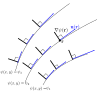
\includegraphics[width=0.75\textwidth]{./psi_streamlines}
 \caption{Relazione tra il campo e la funzione di corrente per un campo di velocità piano che soddisfa il vincolo di incomprimibilità. Il gradiente della funzione di corrente è perpendicolare in ogni punto al vettore velocità e, di conseguenza, le isolinee della funzione di corrente coincidono con le linee di corrente del campo di velocità.}\label{fig:streaml}
\end{figure}

\clearpage \newpage

\section{Tensore degli sforzi}


Il tensore degli sforzi $\mathbb{T}$ è un tensore del secondo ordine che descrive lo stato di sforzo all'interno del mezzo continuo e permette di legare il vettore sforzo $\bm{t_n}$ agente su una superficie elementare e il versore normale $\bh{n}$ alla superficie.
Si considera in un mezzo continuo non polare\footnote{
 All'interno del mezzo continuo, le particelle adiacenti si scambiano unicamente forze elementari, non momenti.
}, e si ricava il legame tra i vettori $\bm{t_n}$, $\bh{n}$ dalle condizioni di equilibrio del tetraedro di Cauchy. Siano $\bh{x}$, $\bh{y}$ e $\bh{z}$ i versori di un sistema di riferimento cartesiano centrato nel punto del continuo considerato e $\bm{t_x}$, $\bm{t_y}$ e $\bm{t_z}$ i vettori sforzo agenti sulle facce del tetraedro di area $dS_x$, $dS_y$ e $dS_z$ con le normali orientate come i rispettivi versori della base, come rappresentato in figura \ref{fig:tetraedroCauchy}. Sia $\bm{t_n}$ il vettore sforzo agente sulla faccia ``inclinata'' di area $dS$ del tetraedro di Cauchy, con normale $\bh{n}$.

\begin{figure}[h!]
\centering
 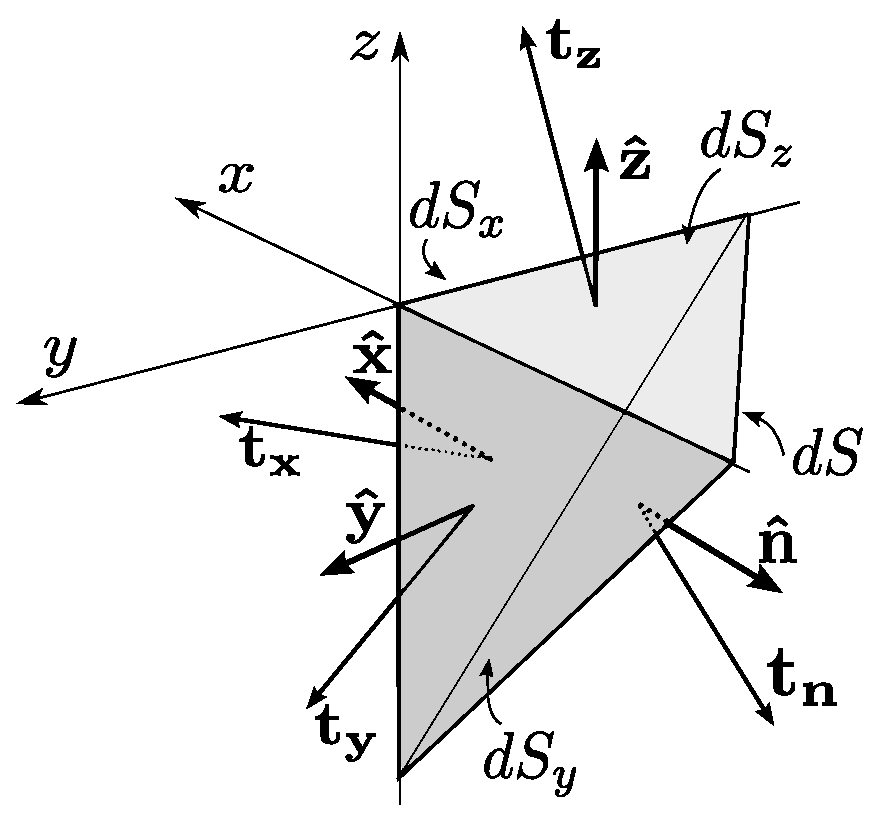
\includegraphics[width=0.60\textwidth]{./fig/cauchy}
\caption{tetraedro di Cauchy}\label{fig:tetraedroCauchy}
\end{figure}

Il legame tra le aree delle facce del tetraedro è
\begin{equation}\label{eqn:surfaces}
 dS = - \dfrac{dS_x}{n_x} = - \dfrac{dS_y}{n_y} = - \dfrac{dS_z}{n_z} ,
\end{equation}
avendo indicato con $n_i$ le componenti cartesiane del versore normale $\bh{n}$, tutte negative per come è stato definito il tetraedro.
Scriviamo il bilancio di massa e di quantità di moto del volume di controllo elementare $dV$ contenuto all'interno del tetraedro di Cauchy. Il bilancio di massa
\begin{equation}
 \f{d}{dt} \int_{dV} \rho + \oint_{\partial dV} \rho \bm{u} \cdot \bh{n} = 0 \ ,
\end{equation}
diventa
\begin{equation}\label{eqn:dV:mass}
\begin{aligned}
 0 = & \p{}{t}\big( \rho + O(d\ell) \big) dV
     + \big( \rho \bm{u} \cdot \bh{x} + O(d\ell) \big) dS_x
     + \big( \rho \bm{u} \cdot \bh{y} + O(d\ell) \big) dS_y \\
   & + \big( \rho \bm{u} \cdot \bh{z} + O(d\ell) \big) dS_z
     + \big( \rho \bm{u} \cdot \bh{n} + O(d\ell) \big) dS \ ,
\end{aligned}
\end{equation}
avendo scritto esplicitamente la dipendenza delle grandezze nel volume e sulle superfici da infinitesimi di ordine $O(d\ell)$, essendo $O(d\ell)$ l'ordine di grandezza delle dimensioni lineari del tetraedro di Cauchy, come ad esempio la lunghezza degli spigoli. Le superfici hanno ordine $O(dS) = O(d\ell^2)$, mentre il volume ha ordine $O(dV) = O(d\ell^3)$. Utilizzando le relazioni (\ref{eqn:surfaces}), facendo tendere $d\ell$ a zero, trascurando gli ifninitesimi di ordine superiore, i termini di ordine $O(d\ell^2)$ si riducono all'identità
\begin{equation}
 \bm{u} \cdot \bh{n} = u_x n_x + u_y n_y + u_z \ .
\end{equation}
Il bliancio di quantità di moto per il tetraedro di Cauchy
\begin{equation}
 \f{d}{dt} \int_V \rho \bm{u} + \oint_{\partial dV} \rho \bm{u} \bm{u} \cdot \bh{n} = \int_{dV} \rho \bm{g} + \oint_{\partial dV} \bm{t_n} \ ,
\end{equation}
diventa
\begin{equation}
\begin{aligned}
 & \p{}{t} \big( \rho \bm{u} + O(d\ell) \big)dV +
 \sum_{i \in \{x,y,z\}} \big( \rho \bm{u} \bm{u} \cdot \bh{x}_i + O(d\ell) \big)dS_i +
                \big( \rho \bm{u} \bm{u} \cdot \bh{n}   + O(d\ell) \big)dS   = \\
 & = \big( \rho \bm{g} + o(d\ell) \big) dV +
     \big( \bm{t_x} + O(d\ell) \big) dS_x +
     \big( \bm{t_y} + O(d\ell) \big) dS_y + \\
 & \hspace{4.5cm} + \big( \bm{t_z} + O(d\ell) \big) dS_z +
     \big( \bm{t_n} + O(d\ell) \big) dS \ .
\end{aligned}
\end{equation}
I termini ``più grandi'' sono infinitesimi di ordine $O(d\ell^2)$.
Utilizzando il bilancio di massa, non è difficile verificare che i termini di flusso di quantità di moto danno un contributo nullo di ordine $O(d\ell^2)$. I termini di volume sono infinitesimi di ordine $O(d\ell^3)$.
Facendo tendere $d\ell$ a zero e trascurando tutti gli infinitesimi di ordine superiore a $O(d\ell)$ si ottiene
\begin{equation}\label{eqn:dV:equil}
\begin{aligned}
 \bm{0} & = \bm{t_n} dS + \bm{t_x} dS_x + \bm{t_y} dS_y + \bm{t_z} dS_z = \\
  & = ( \bm{t_n} - \bm{t_x} n_x - \bm{t_y} n_y - \bm{t_z} n_z ) dS  \qquad \rightarrow \qquad \bm{t_n} = \bm{t_x} n_x + \bm{t_y} n_y + \bm{t_z} n_z \ .
\end{aligned}
\end{equation}
Se si esprimono i vettori utilizzando la base $\{\bh{x}, \, \bh{y}, \, \bh{z} \}$,
\begin{equation}\label{eqn:t:comp}
  \bm{t_i} = t_{ix} \bh{x} + t_{iy} \bh{y} + t_{iz} \bh{z} \ ,
\end{equation}
si può scrivere la relazione (\ref{eqn:dV:equil}) per trovare la relazione tra il versore $\bh{n}$ e il vettore sforzo $\bm{t_n}$
\begin{equation}
\begin{aligned}
  \bm{t_n} & = \bm{t_x} n_x + \bm{t_y} n_y + \bm{t_z} n_z \\ 
 & = n_x ( t_{xx} \bm{\hat{x}} + t_{xy} \bm{\hat{y}} +  t_{xz} \bm{\hat{z}} ) % + \\
   + n_y ( t_{yx} \bm{\hat{x}} + t_{yy} \bm{\hat{y}} +  t_{yz} \bm{\hat{z}} ) % + \\
   + n_z ( t_{zx} \bm{\hat{x}} + t_{zy} \bm{\hat{y}} +  t_{zz} \bm{\hat{z}} ) = \\
 & = ( \bh{n} \cdot \bh{x} ) ( t_{xx} \bm{\hat{x}} + t_{xy} \bm{\hat{y}} +  t_{xz} \bm{\hat{z}} )% + \\
   + ( \bh{n} \cdot \bh{y} ) ( t_{yx} \bm{\hat{x}} + t_{yy} \bm{\hat{y}} +  t_{yz} \bm{\hat{z}} )% + \\
   + ( \bh{n} \cdot \bh{z} ) ( t_{zx} \bm{\hat{x}} + t_{zy} \bm{\hat{y}} +  t_{zz} \bm{\hat{z}} ) = \\
%   & = ( \bm{n} \cdot \bm{\hat{x}} ) \bm{t_x} + 
%       ( \bm{n} \cdot \bm{\hat{y}} ) \bm{t_y} + 
%       ( \bm{n} \cdot \bm{\hat{z}} ) \bm{t_z} = \\
    & = \bh{n} \cdot ( t_{xx} \bm{\hat{x}} \otimes \bm{\hat{x}} + 
                       t_{xy} \bm{\hat{x}} \otimes \bm{\hat{y}} +
                       t_{xz} \bm{\hat{x}} \otimes \bm{\hat{z}} + \\
            & \qquad + t_{yx} \bm{\hat{y}} \otimes \bm{\hat{x}} + 
                       t_{yy} \bm{\hat{y}} \otimes \bm{\hat{y}} +
                       t_{yz} \bm{\hat{y}} \otimes \bm{\hat{z}} + \\
            & \qquad + t_{zx} \bm{\hat{z}} \otimes \bm{\hat{x}} + 
                       t_{zy} \bm{\hat{z}} \otimes \bm{\hat{y}} +
                       t_{zz} \bm{\hat{z}} \otimes \bm{\hat{z}} ) =
     \bm{\hat{n}} \cdot \mathbb{T}  \ ,
\end{aligned}  
\end{equation}
avendo utilizzato l'identità $(\bm{a} \cdot \bm{b})\bm{c} = \bm{a} \cdot (\bm{b}\otimes\bm{c})$, per isolare il versore $\bh{n}$ dal tensore degli sforzi $\mathbb{T}$. Avendo utilizzato la definizione (\ref{eqn:t:comp}) delle componenti cartesiane dei vettori dello sforzo agente sulle facce del tetraedro di Cauchy, il primo indice delle componenti del tensore degli sforzi indica la faccia sulla quale agisce lo sforzo, il secondo indice la sua componente cartesiana, cosicché la componente $t_{ij}$ indica la componente cartesiana $j$-esima agente sulla $i$-esima faccia del tetraedro di Cauchy.
%
\newline \noindent
\textbf{Osservazione 1.} Utilizzando le convenzioni scelte in precedenza, il vettore sforzo si ottiene con la relazione
\begin{equation}
 \bm{t_n} = \bh{n} \cdot \mathbb{T} \qquad , \qquad t_{n,i} = n_j t_{ji} \ ,
\end{equation}
che in generale differisce dall'operazione $\mathbb{T} \cdot \bh{n}$, la cui $i$-esima componente cartesiana è $n_j t_{ij}$.
%
\newline \noindent
\textbf{Osservazione 2.} Se il tensore $\mathbb{S}$ è simmetrico (e quindi le sue componenti con indici misti sono uguali, $S_{ij} = S_{ji}$), la moltiplicazione a sinista o a destra di un vettore tramite il prodotto ``punto'' dà lo stesso risultato,
\begin{equation}
 \bm{a} \cdot \mathbb{S} = \mathbb{S} \cdot \bm{a} \qquad , \qquad 
 a_j S_{ji} = S_{ij} a_j \ .
\end{equation}
%
\newline \noindent
\textbf{Osservazione 3.} Il tensore degli sforzi per mezzi continui non polari è simmetrico. Questo permette di ottenere la corretta relazione tra versore normale alla superficie e vettore sforzo, anche in seguito ad alcune imprecisioni nell'utilizzo delle operazioni tensoriali, come uno scambio di indici nel tensore degli sforzi.
%
\newline \noindent
\textbf{Osservazione 4.} Non è stata prestata mai attenzione alla posizione degli indici poiché si è lavorato sempre con basi ortonormali, come la base cartesiana.
%
\newline \noindent
\textbf{Osservazione 5.} \'E possibile utilizzare altre convenzioni nella definizione delle componenti dei vettori sforzo agenti sulle facce del tetraedro di Cauchy, che portano a una diversa interpretazione degli indici e alla rappresentazione della relazione di Cauchy.





\clearpage \newpage

\section{Equazione della quantità di moto e curvatura delle linee di corrente}

L'equazione della quantità di moto è
\begin{equation}
 \rho \left\{ \frac{\partial \bm{u}}{\partial t} +
   \left( \bm{u} \cdot \bm{\nabla} \right) \bm{u} \right\} = 
   \bm{\nabla} \cdot \mathbb{T} + \bm{f}
\end{equation}
dove con $\mathbb{T}$ è stato indicato il tensore degli sforzi,
 che per un fluido newtoniano è $\mathbb{T} = -p \mathbb{I} + \mathbb{S}$
 con $\mathbb{S} = 2 \mu \mathbb{D} + \lambda \left( 
 \bm{\nabla} \cdot \bm{u} \right) \mathbb{I}$ e $\mathbb{D} = \frac{1}{2}
 \left[ \bm{\nabla}\bm{u} + \bm{\nabla}^T \bm{u} \right]$ il tensore
 velocità di deformazione, parte simmetrica del gradiente della velocità.
%
Introducendo la derivata materiale, si ritrova una forma ``familiare''
 del secondo principio della dinamica
\begin{equation}
 \rho\frac{D\bm{u}}{D t} = \bm{\nabla} \cdot \mathbb{T} + \bm{f}
  \qquad \Rightarrow \qquad
 \rho\bm{a} = \bm{\nabla} \cdot \mathbb{T} + \bm{f}
\end{equation}
%
\paragraph{Richiami di geometria delle curve nello spazio.}
Una curva è un luogo di punti che può essere parametrizzato tramite un
 parametro solo.
La parametrizzazione $\bm{r}(t)$ della curva $\bm{r}$ è definita regolare 
 se $d\bm{r}/dt \ne 0$. Si definisce poi una parametrizzazione regolare
 particolare, l'ascissa curvilinea $s$ tale per cui $\left| d\bm{r}(s)/ds
 \right| = 1, \forall s \in (a,b)$.

\noindent 
Nel seguito si introduce brevemente la \textbf{terna di Frenet} 
 $\left\{\bm{\hat{t}}, \bm{\hat{n}}, \bm{\hat{b}} \right\}$, formata
 dai versori tangente, normale e binormale, in funzione dell'ascissa
 curvilinea.
%
Si dimostra che
\begin{equation}
 \bm{\hat{t}}(s) = \dfrac{d\bm{r}}{ds}
\end{equation}
%
La derivata seconda della posizione $\bm{r}$, cioè la derivata prima del
 versore tangente $\bm{\hat{t}}$ è legata al versore normale
 $\bm{\hat{t}}$, tramite la curvatura $k = \left| \frac{d\bm{\hat{t}}}{
 ds} \right|$.
\begin{equation}
 \bm{\hat{n}} = \dfrac{\frac{d\bm{\hat{t}}}{ds}}
    {\left|\frac{d\bm{\hat{t}}}{ds} \right|} 
  \qquad \Rightarrow \qquad
 \dfrac{d\bm{\hat{t}}}{ds} = k \bm{\hat{n}}
\end{equation}
%
Il versore binormale è definito a completare la terna ortonormale 
 destrorsa
\begin{equation}
 \bm{\hat{b}} = \bm{\hat{t}} \times \bm{\hat{n}} 
\end{equation}
%
Per completezza e senza troppo sforzo si calcolano anche le derivate 
 di tali versori, ricordando che hanno modulo unitario e costante,
 e formano una terna ortogonale in ogni punto, introducendo la definizione
 della torsione $\tau = \frac{d \bm{\hat{n}}}{ds}\cdot \bm{b}$.
\begin{equation}
\begin{aligned}
& \qquad \qquad \qquad \qquad \qquad \qquad \qquad \qquad 
  \qquad \qquad \qquad \qquad \quad
 \frac{d \bm{\hat{t}}}{ds} = k \bm{\hat{n}} \\
& \begin{cases}
 \bm{\hat{n}}'\cdot \bm{\hat{n}} = 0 \\
 \bm{\hat{n}}'\cdot \bm{\hat{t}}+\bm{\hat{t}}'\cdot \bm{\hat{n}} = 0 \\
 \bm{\hat{n}}'\cdot \bm{\hat{b}} = \tau \\
 \end{cases} \Rightarrow \quad
 \begin{cases}
 \bm{\hat{n}}'\cdot \bm{\hat{n}} = 0   \\
 \bm{\hat{n}}'\cdot \bm{\hat{t}} = -k  \\
 \bm{\hat{n}}'\cdot \bm{\hat{b}} = \tau \\
 \end{cases} \qquad \quad \quad \Rightarrow \quad 
  \frac{d \bm{\hat{n}}}{ds} = - k \bm{\hat{t}} + \tau \bm{\hat{b}} \\
& \begin{cases}
 \bm{\hat{b}}'\cdot \bm{\hat{b}} = 0 \\
 \bm{\hat{b}}'\cdot \bm{\hat{t}} + \bm{\hat{t}}'\cdot \bm{\hat{b}} = 0 \\
 \bm{\hat{b}}'\cdot \bm{\hat{n}} + \bm{\hat{n}}'\cdot \bm{\hat{b}} = 0 \\
 \end{cases} \Rightarrow \quad
 \begin{cases}
 \bm{\hat{b}}'\cdot \bm{\hat{b}} = 0 \\
 \bm{\hat{b}}'\cdot \bm{\hat{t}} = -\bm{\hat{t}}'\cdot \bm{\hat{b}} = 0 \\
 \bm{\hat{b}}'\cdot \bm{\hat{n}} = -\bm{\hat{n}}'\cdot \bm{\hat{b}} = -k\\
 \end{cases} \Rightarrow \quad
  \frac{d \bm{\hat{b}}}{ds} = - \tau \bm{\hat{n}} \\
\end{aligned}
\end{equation}
%
Se la parametrizzazione regolare della curva non è l'ascissa curvilinea,
 si può ricavare
\begin{equation}
 \frac{d\bm{r}}{dt} = \frac{ds}{dt}\frac{d\bm{r}}{ds} = 
  v \bm{\hat{t}}
\end{equation}
dove si è introdotto il modulo $v$ di quella che sarà la velocità $\bm{v}$
 quando $\bm{r}$ e $t$ saranno spazio e tempo.
In maniera analoga
\begin{equation}
 \frac{d\bm{\hat{t}}}{dt} = \frac{ds}{dt}\frac{d\bm{\hat{t}}}{ds} = 
  v k \bm{\hat{n}}
\end{equation}
 %
Se $\bm{r}$ e $t$ sono spazio e tempo, la velocità e l'accelerazione di un
 punto che ha come legge oraria $\bm{r}(t)$ sono
\begin{equation}
 \begin{aligned}
  \bm{v} & = \frac{d\bm{r}}{dt} = \frac{ds}{dt}\frac{d\bm{r}}{ds} = 
    v \bm{\hat{t}} \\
  \bm{a} & = \frac{d\bm{v}}{dt} =
   \frac{dv}{dt} \bm{\hat{t}} + v \frac{d\bm{\hat{t}}}{dt} =
   \frac{dv}{dt} \bm{\hat{t}} + v^2 k \bm{\hat{n}}
 \end{aligned}
\end{equation}
%
\begin{minipage}{0.60\textwidth}
\paragraph{Ritorno al bilancio della quantità di moto.} Inserendo la
 forma dell'accelerazione nell'equazione della quantità di moto e 
 proiettando lungo i versori della terna di Frenet
\begin{equation}
 \begin{cases}
  \rho \frac{dv}{dt} =  \bm{\hat{t}} \cdot \left(
     \bm{\nabla} \cdot \mathbb{T} + \bm{f} \right) \\
  \rho v^2 k = \bm{\hat{n}} \cdot \left(
     \bm{\nabla} \cdot \mathbb{T} + \bm{f} \right) \\
  0 = \bm{\hat{b}} \cdot \left(
     \bm{\nabla} \cdot \mathbb{T} + \bm{f} \right) \\
 \end{cases}
\end{equation}
L'analisi per componenti locali dell'equazione della quantità di moto permette di riconoscere che:
\end{minipage}
\hfill
\begin{minipage}{0.40\textwidth}
\begin{center}
   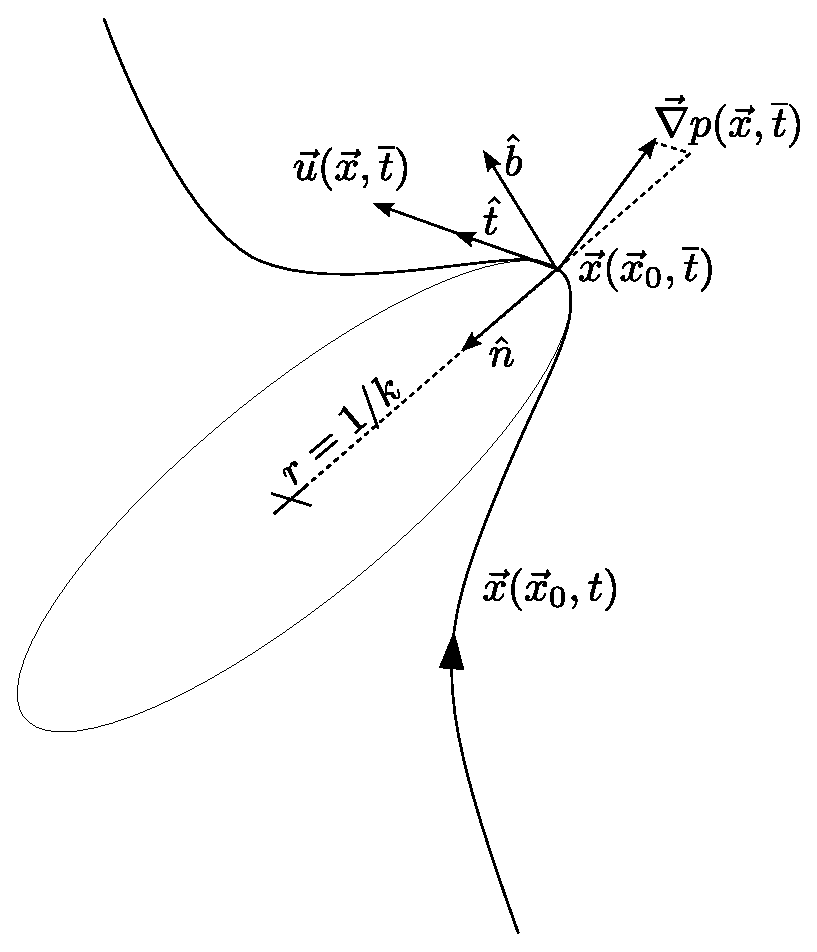
\includegraphics[width=1.0\textwidth]{./fig/frenet.eps}
\end{center}
\end{minipage}
\begin{itemize}
 \item la proiezione del termine forzante lungo la tangente alla traiettoria è la responsabile dell'accelerazione tangenziale della particella materiale;
 \item la proiezione del termine forzante lungo la normale alla traiettoria è la responsabile dell'accelerazione centripeta della particella maetriale e, di conseguenza, della curvatura della traiettoria;
 \item la proiezione della forzante lungo la direzione binormale è nulla.
\end{itemize}

\noindent
In assenza di forze di volume ($\bm{f}=0$) e sforzi viscosi
($\mathbb{T}=\mathbb{S}-p\mathbb{I}=-p\mathbb{I}$):
\begin{equation}
 \begin{cases}
  \rho \frac{dv}{dt} = - \bm{\hat{t}} \cdot \bm{\nabla} p \\
  \rho v^2 k         = - \bm{\hat{n}} \cdot \bm{\nabla} p \\
  0                  = - \bm{\hat{b}} \cdot \bm{\nabla} p \\
 \end{cases}
\end{equation}
%
e quindi:
\begin{itemize}
 \item l'accelerazione tangenziale è proporzionale alla proiezione del gradiente di pressione in direzione tangente alla tratiettoria;
 \item l'accelerazione centripeta, $v^2/r = v^2 k$, è proporzionale alla proiezione del gradiente di pressione in direzione normale alla tratiettoria. Il termine $\rho v^2 k$ è sempre positivo poichè prodotto di quantità positive: la curvatura di una linea è non negativa per come è definita, la densità è positiva, il modulo di un vettore è anch'esso non negativo. Il prodotto scalare tra la normale e il gradiente della pressione (derivata direzionale della pressione in direzione $\bm{\hat{n}}$) deve quindi essere negativo. La pressione quindi diminuisce, andando verso il centro del cerchio osculatore. Sempre dalla seconda equazione è immediato notare che la curvatura della traiettoria è proporzionale alla componente del gradiente di pressione lungo il versore normale;
 \item la proiezione del gradiente di pressione in direzione binormale a una traiettoria è nullo.
\end{itemize}
% Un'analisi della componente normale permette di ricavare, \textbf{sotto le
%  ipotesi fatte}, il legame tra la curvatura delle traiettorie delle
%  particelle fluide e il gradiente del campo di pressione.
% Il termine a sinistra dell'uguale è positivo
% La componente tangente fa aumentare 
%  il modulo della velocità, mentre la componente binormale deve essere nulla.
%Essendo il versore $\bm{\hat{n}}$ diretto verso il centro del cerchio
% osculatore (in parole povere è diretta verso l'interno della curva),
% la curvatura $k$ positiva, segue che la pressione deve diminuire lungo 
% $\bm{\hat{n}}$, cioè aumenta all'allontanarsi dal cerchio del centro
% osculatore (in parole altrettanto povere, ``verso l'esterno'').
%\textit{(Nemmeno a dirlo, la densità $\rho$ è positiva e il quadrato
%  del modulo della velocità $v^2$ è positivo.)}
%\noindent
%Dalla componente lungo $\bm{\hat{n}}$ si nota che il legame tra 
% la componente del gradiente della pressione in quella direzione è
% \textbf{proporzionale} alla curvatura della traiettoria della particella
% fluida.


\clearpage \newpage

\section{Teoremi di Bernoulli ed equazione della vorticità}
Per fluidi incomprimibili o barotropici (per i quali la pressione è funzione solo della densità), il teorema di Bernoulli si ottiene dal bilancio della quantità di moto. Si elencano qui tre forme del teorema di Bernoulli, ognuna caratterizzata da diverse ipotesi.
%
Tramite l'identità vettoriale
\begin{equation}
  \bm{\nabla} (\bm{a} \cdot \bm{b}) = (\bm{a} \cdot \bm{\nabla}) \bm{b} +  (\bm{b} \cdot \bm{\nabla}) \bm{a} + \bm{a} \times (\bm{\nabla} \times \bm{b}) + \bm{b} \times (\bm{\nabla} \times \bm{a}),
\end{equation}
applicata al termine convettivo $(\bm{u} \cdot \bm{\nabla}) \bm{u}$, è possible ottenere la forma del Crocco dell'equazione della quantità di moto
\begin{equation}\label{eqn:bilanci:crocco}
\begin{aligned}
 & \p{\bm{u}}{t} + (\bm{u} \cdot \bm{\nabla}) \bm{u} - \nu \Delta \bm{u} + \bm{\nabla} P = \bm{g}  & \\ &  &  \bigg( (\bm{u} \cdot \bm{\nabla})\bm{u} = \bm{\nabla} \f{\bm{u} \cdot \bm{u}}{2} + (\bm{\nabla} \times \bm{u}) \times \bm{u} \bigg) \\
 & \rightarrow \p{\bm{u}}{t} + \bm{\nabla} \frac{|\bm{u}|^2}{2} + \bm{\omega} \times \bm{u} - \nu \Delta \bm{u} + \bm{\nabla} P = \bm{g} , & \\
\end{aligned}
\end{equation}
avendo indicato con $P$ il potenziale termodinamico, $P = $ che si riduce al rapporto $p/\rho$ nel caso di densità costante e con $\bm{g}$ le forze per unità di massa.
\paragraph{Prima forma del teorema di Bernoulli}
Nel caso di fluido non viscoso, incomprimibile o barotropico, in regime stazionario ($\partial / \partial t \equiv 0$), con forze di massa conservative $\bm{g} = -\bm{\nabla} \chi$, il trinomio di Bernoulli $|\bm{u}|^2/2 + P + \chi$ è costante lungo le linee di corrente e le linee vorticose, cioè
\begin{equation}
 \bm{\hat{t}} \cdot \bm{\nabla} \left( \frac{|\bm{u}|^2}{2} + P + \chi \right) = 0 ,
\end{equation}
con $\bm{\hat{t}}$ versore tangente alle linee di corrente o alle linee vorticose. Infatti, il termine $\bm{\omega} \times \bm{u}$ nell'equazione della quantità di moto nella forma di Crocco (\ref{eqn:bilanci:crocco}) è perpendicolare in ogni punto del dominio alle linee di corrente ($\bm{\hat{t}}$ parallelo al campo di velocità $\bm{u}$) e alle linee vorticose ($\bm{\hat{t}}$ parallelo al campo di vorticità $\bm{\omega}$): moltiplicando scalarmente l'equazione (\ref{eqn:bilanci:crocco}) scritta per un fluido non viscoso ($\nu = 0$) per il versore $\bm{\hat{t}}$ , il prodotto scalare $\bm{\hat{t}} \cdot (\bm{\omega} \times \bm{u})$ è identicamente nullo.
\paragraph{Seconda forma del teorema di Bernoulli}
Nella corrente irrotazionale ($\bm{\omega} = \bm{0}$) di un fluido non viscoso, incomprimibile o barotropico, in regime stazionario, con forze di massa conservative $\bm{g} = -\bm{\nabla} \chi$, il trinomio di Bernoulli $|\bm{u}|^2/2 + P + \chi$ è costante in tutto il dominio, cioè
\begin{equation}
 \bm{\nabla} \left( \frac{|\bm{u}|^2}{2} + P + \chi \right) = 0  \quad \rightarrow \quad 
  \frac{|\bm{\nabla} \phi|^2}{2} + P + \chi = C.
\end{equation}
\paragraph{Terza forma del teorema di Bernoulli}
Nella corrente irrotazionale ($\bm{\omega} = \bm{0}$) di un fluido non viscoso, incomprimibile o barotropico, in un dominio semplicemente connesso (nel quale è quindi possibile definire il potenziale cinetico $\phi$, t.c. $\bm{u} = \nabla \phi$, con forze di massa conservative $\bm{g} = -\bm{\nabla} \chi$, il quadrinomio di Bernoulli $\partial \phi / \partial t + |\bm{u}|^2/2 + P + \chi$ è uniforme (costante in spazio, in generale \textbf{non} in tempo) in tutto il dominio, cioè
\begin{equation}
 \bm{\nabla} \left(\p{\phi}{t} + \frac{|\bm{\nabla} \phi|^2}{2} + P + \chi \right) = 0  \quad \rightarrow \quad 
 \p{\phi}{t} + \frac{|\bm{\nabla} \phi|^2}{2} + P + \chi = C(t).
\end{equation}

\paragraph{Teoremi di Bernoulli per fluidi viscosi incomprimibili}
Mentre la prima forma del teorema di Bernoulli non è valida se non viene fatta l'ipotesi di fluido non viscoso\footnote{Moltiplicando scalarmente l'equazione (\ref{eqn:bilanci:crocco}) per il versore $\bm{\hat{t}}$, il termine $\bm{\hat{t}}\cdot \nu \Delta \bm{u}$ non si annulla. Rimane quindi
\begin{equation}
 \bm{\hat{t}} \cdot \bm{\nabla} \left( \frac{|\bm{u}|^2}{2} + P + \chi \right) - \nu \bm{\hat{t}} \cdot \Delta \bm{u} = 0 
\end{equation}
}, la seconda e la terza forma sono ancora valide per fluidi viscosi incomprimibili. Infatti, usando l'identità vettoriale
\begin{equation}
 \Delta \bm{u} = \bm{\nabla} (\bm{\nabla}\cdot \bm{u})
  - \bm{\nabla} \times (\bm{\nabla} \times \bm{u}) ,
\end{equation}
si scopre che il laplaciano del campo di velocità per correnti irrotazionali ($\bm{\nabla} \times \bm{u} = \bm{0}$) di fluidi incomprimibili ($\bm{\nabla} \cdot \bm{u} = 0$) è nullo.
%
\begin{remark}
L'ipotesi di fluido non viscoso non è direttamente necessaria per la seconda e la terza forma del teorema di Bernoulli, ma lo diventa tramite l'ipotesi di corrente irrotazionale. Sotto opportune ipotesi sulla corrente asintotica, verificate in molti casi di interesse aeronautico, si dimostra che (quasi) tutto il campo di moto è  irrotazionale solo se viene fatta l'ipotesi di fluido non viscoso. Questo modello viene utilizzato per studiare correnti di interesse aeronautico, nelle quali gli effetti della viscosità sono (quasi ovunque) trascurabili: un esempio è la corrente, uniforme a monte, che investe un corpo aerodinamico a bassi angoli di incidenza (corpo affusolato, attorno al quale non si verifichino separazioni) per alti numeri di Reynolds: in queste correnti, le zone vorticose sono confinate in regioni di spessore sottile (strato limite sulla superficie dei corpi solidi e scie libere).
\end{remark}





\clearpage \newpage




\end{document}
